% generated by paper/scripts/make_tables.py -- do not edit by hand
\begin{figure}[t]
\centering
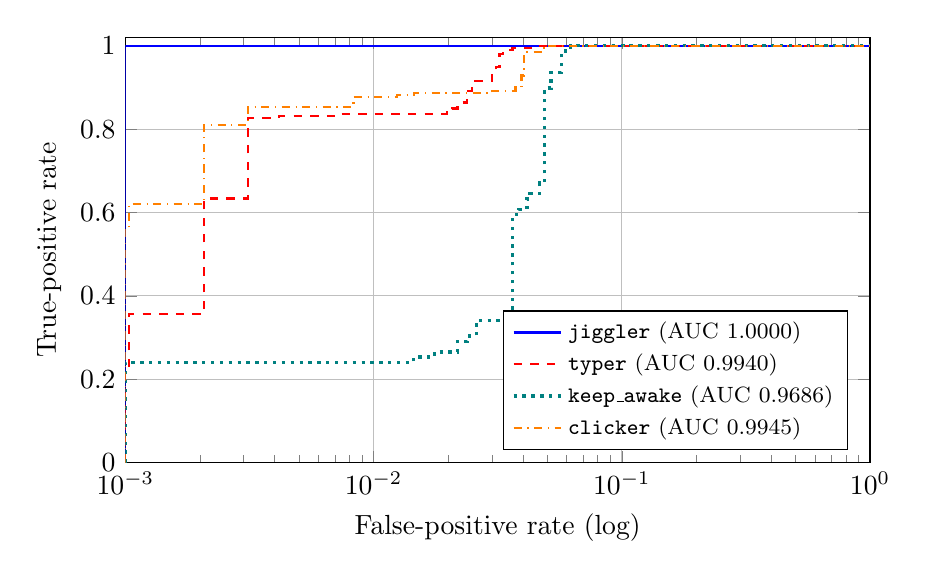
\begin{tikzpicture}
\begin{axis}[
  width=0.78\columnwidth, height=5.4cm, scale only axis,
  xmode=log, xmin=0.001, xmax=1, ymin=0, ymax=1.02,
  xlabel={False-positive rate (log)}, ylabel={True-positive rate},
  grid=major, legend pos=south east, legend cell align=left,
  legend style={font=\footnotesize},
]
\addplot[solid, color=blue, thick] coordinates {(0.001,0) (0.001,0.007042) (0.001,0.03521) (0.001,0.07042) (0.001,0.1197) (0.001,0.1338) (0.001,0.2113) (0.001,0.2254) (0.001,0.4577) (0.001,0.5352) (0.001,0.6408) (0.001,0.6831) (0.001,0.7183) (0.001,0.7324) (0.001,0.7676) (0.001,0.7958) (0.001,0.8028) (0.001,0.831) (0.001,0.8451) (0.001,0.8732) (0.001,0.9507) (0.001,0.9859) (0.001,1) (0.01037,1) (0.01245,1) (0.05705,1) (0.05913,1) (0.08817,1) (0.09129,1) (0.09232,1) (0.0944,1) (0.09544,1) (0.1017,1) (0.1037,1) (0.1079,1) (0.1089,1) (0.111,1) (0.1151,1) (0.1172,1) (0.1183,1) (0.1224,1) (0.1234,1) (0.1255,1) (0.1266,1) (0.1369,1) (0.1535,1) (1,1)};
\addlegendentry{\texttt{jiggler} (AUC 1.0000)}
\addplot[dashed, color=red, thick] coordinates {(0.001,0) (0.001,0.004695) (0.001,0.05164) (0.001,0.06103) (0.001,0.07042) (0.001,0.07981) (0.001,0.0939) (0.001,0.1221) (0.001,0.1315) (0.001,0.1408) (0.001,0.169) (0.001,0.1784) (0.001,0.1831) (0.001,0.2066) (0.001,0.216) (0.001037,0.216) (0.001037,0.2582) (0.001037,0.2676) (0.001037,0.2723) (0.001037,0.2864) (0.001037,0.3099) (0.001037,0.3192) (0.001037,0.3568) (0.002075,0.3568) (0.002075,0.3662) (0.002075,0.3803) (0.002075,0.3897) (0.002075,0.3944) (0.002075,0.4085) (0.002075,0.4131) (0.002075,0.4319) (0.002075,0.4507) (0.002075,0.4977) (0.002075,0.5258) (0.002075,0.554) (0.002075,0.5728) (0.002075,0.6103) (0.002075,0.6338) (0.003112,0.6338) (0.003112,0.6526) (0.003112,0.6667) (0.003112,0.6761) (0.003112,0.6854) (0.003112,0.7089) (0.003112,0.7183) (0.003112,0.7418) (0.003112,0.7559) (0.003112,0.7746) (0.003112,0.7887) (0.003112,0.8028) (0.003112,0.8169) (0.003112,0.8263) (0.004149,0.8263) (0.004149,0.831) (0.007261,0.831) (0.007261,0.8357) (0.009336,0.8357) (0.01141,0.8357) (0.01971,0.8357) (0.01971,0.8404) (0.02075,0.8404) (0.02075,0.8498) (0.02178,0.8498) (0.02178,0.8638) (0.02386,0.8638) (0.02386,0.8732) (0.02386,0.892) (0.0249,0.892) (0.0249,0.9014) (0.0249,0.9155) (0.03008,0.9155) (0.03008,0.9202) (0.03008,0.9296) (0.03112,0.9296) (0.03112,0.9343) (0.03112,0.9484) (0.03216,0.9484) (0.03216,0.9765) (0.03216,0.9812) (0.0332,0.9812) (0.0332,0.9906) (0.03631,0.9906) (0.03631,0.9953) (0.04461,0.9953) (0.04461,1) (0.07573,1) (0.0778,1) (0.07988,1) (0.08299,1) (0.0861,1) (0.09025,1) (0.1027,1) (0.1048,1) (0.1255,1) (0.1338,1) (0.1359,1) (0.1369,1) (0.1411,1) (0.1525,1) (1,1)};
\addlegendentry{\texttt{typer} (AUC 0.9940)}
\addplot[dotted, color=teal, very thick] coordinates {(0.001,0) (0.001,0.01266) (0.001,0.02532) (0.001,0.05063) (0.001,0.2405) (0.009336,0.2405) (0.01141,0.2405) (0.01452,0.2405) (0.01452,0.2532) (0.01763,0.2532) (0.01763,0.2658) (0.02178,0.2658) (0.02178,0.2911) (0.02386,0.2911) (0.02386,0.3038) (0.02593,0.3038) (0.02593,0.3418) (0.03631,0.3418) (0.03631,0.5949) (0.03838,0.5949) (0.03838,0.6076) (0.04149,0.6076) (0.04149,0.6329) (0.04253,0.6329) (0.04253,0.6456) (0.04668,0.6456) (0.04668,0.6709) (0.04876,0.6709) (0.04876,0.8987) (0.05187,0.8987) (0.05187,0.9367) (0.05394,0.9367) (0.05602,0.9367) (0.05705,0.9367) (0.05705,0.9494) (0.05705,0.9873) (0.06224,0.9873) (0.06224,1) (0.07054,1) (0.07261,1) (0.08091,1) (0.08299,1) (0.08921,1) (0.09129,1) (0.09959,1) (0.1017,1) (0.1048,1) (0.1089,1) (0.111,1) (0.1203,1) (0.1224,1) (0.1411,1) (0.1452,1) (0.1712,1) (0.1732,1) (0.1743,1) (1,1)};
\addlegendentry{\texttt{keep\_awake} (AUC 0.9686)}
\addplot[dashdotted, color=orange, thick] coordinates {(0.001,0) (0.001,0.004739) (0.001,0.2085) (0.001,0.218) (0.001,0.4076) (0.001,0.4171) (0.001,0.4597) (0.001,0.4692) (0.001,0.5355) (0.001,0.5545) (0.001,0.564) (0.001037,0.564) (0.001037,0.5687) (0.001037,0.5782) (0.001037,0.5972) (0.001037,0.6066) (0.001037,0.6209) (0.002075,0.6209) (0.002075,0.6351) (0.002075,0.6445) (0.002075,0.6588) (0.002075,0.6967) (0.002075,0.7251) (0.002075,0.7393) (0.002075,0.7488) (0.002075,0.7583) (0.002075,0.7678) (0.002075,0.7725) (0.002075,0.8104) (0.003112,0.8104) (0.003112,0.8294) (0.003112,0.8436) (0.003112,0.8531) (0.008299,0.8531) (0.008299,0.8578) (0.008299,0.872) (0.008299,0.8768) (0.01245,0.8768) (0.01245,0.8815) (0.01452,0.8815) (0.01452,0.8863) (0.03008,0.8863) (0.03008,0.891) (0.03734,0.891) (0.03734,0.9005) (0.03942,0.9005) (0.03942,0.9194) (0.03942,0.9289) (0.04046,0.9289) (0.04046,0.9384) (0.04046,0.9526) (0.04046,0.9716) (0.04046,0.9763) (0.04149,0.9763) (0.04149,0.9858) (0.04357,0.9858) (0.04772,0.9858) (0.04772,0.9953) (0.04979,0.9953) (0.04979,1) (0.05187,1) (0.06017,1) (0.06224,1) (0.06639,1) (0.06846,1) (0.07158,1) (0.08091,1) (0.08299,1) (0.08714,1) (0.08921,1) (0.09336,1) (0.09544,1) (0.09647,1) (0.09959,1) (0.1037,1) (0.1214,1) (0.1276,1) (0.1286,1) (0.1369,1) (0.14,1) (1,1)};
\addlegendentry{\texttt{clicker} (AUC 0.9945)}
\end{axis}
\end{tikzpicture}
\caption{ROC curves of the leave-one-kind-out folds of
Table~\ref{tab:crosskind}, on a logarithmic false-positive axis
(false-positive rates of zero are clipped to $10^{-3}$). Every fold ranks
the classes almost perfectly, including the \texttt{typer} fold whose
$F_1$ at the fixed threshold is zero: the failure is calibration, not
separability.}
\label{fig:roc}
\end{figure}
